\chapter{Experiment on RE}
Trough out this thesis, I was interested in a strategy of referencing, where the first reference does not always uniquely identifies the target object. Instead, the strategy relied on a feedback and additional references, which together with the first reference formed a chain of references. I wondered what is the effect of this splitting of the information across more references. In Chapter \ref{chap:ml} this strategy was explored through phenomenon of chains of references. After not being able to model this behaviour through methods of machine learning, I decided to look at that strategy under more controlled conditions of an experiment.

In the first section, I'll present my hypothesis concerning the strategy of splitting references. 

The second section will describe the experimental set-up. 

In the last section, I'll summarize the results of the experiment.

\section{Hypothesis}
To evaluate strategy of splitting references, I compared two NLG systems, which I have built to resemble human IGs from the S-GIVE dataset. The two systems are identical, except for a difference in a REG strategy for the target button. One system represents the strategy of splitting references, while the other one would represent more standard approach of referencing. They will be thoroughly described in Section \ref{sec:exper-setup}.

The question this chapter tries to answer is how splitting references affects the task proficiency. Is this strategy significantly different from more of standard fully-identifying reference? Or is it simply a language device IG can utilize in complicated virtual worlds.

I've formulated my prediction to these questions as hypothesis:

\begin{hypo}
Distributing information to uniquely identify the referent across multiple referring expressions separated by non-negligible time intervals does not have an impact on the task proficiency.
\end{hypo}

%\begin{alterhypo}
%Distributing information to uniquely identify the referent across multiple referring %expressions separated by non-negligible time intervals does not have an impact on the %task proficiency.
%\end{alterhypo}

Measuring task proficiency can be done in several ways. In previous chapters, I've often employed duration of the experiment. However, for this experiment I've chosen more specific measure, in order to diminish effects of other factors. I've measured time from the point of uttering the first reference up to the pressing of the targeted button. This not only diminishes effects of other variables in the navigation process, but can also be interpreted as a measure how well were the references understood by IF.

For testing the hypothesis I've compared the average times between the first reference and the pressing of the target button for both systems. I've used independent two-sample t-test for unequal sample size. The unequal sample size comes from the fact that the subject could press a wrong button and therefore the number of potential references may vary.

Having formulated hypothesis and translating it into statistical test, I can now describe how I approached setting up the experiment.

\section{Experimental set-up}
\label{sec:exper-setup}
I've tested my hypothesis through a human subjects evaluation. Each subject did 5 virtual worlds from GIVE scenario. One of the worlds was a short tutorial world. This tutorial world was excluded from the analysis and served the purpose of diminishing the effect of learning. After the tutorial world, the subjects did 4 evaluation worlds in a random order. The two tested NLG systems were assigned to each world semi-randomly to ensure both of the systems appeared twice. Please note, that the tutorial world was created in such way that the two tested NLG systems behaved the same way and therefore none of the systems had an advantage in number of trials. I've used text instruction presented on the screen as in the GIVE Challenge instalments. Using some sort of speech synthesis or even recorded instructions was beyond the scope of this thesis.

The worlds were similar to the GIVE challenge worlds. Maps generated by GIVE map-viewer for all of the 4 evaluation worlds can be found in Figures \ref{fig:exper-world1}, \ref{fig:exper-world2}, \ref{fig:exper-world3} and \ref{fig:exper-world4}. I did not include any alarm tiles or alarm-causing buttons in the worlds, to avoid situation where IF would loose. I also avoided complex arrays of buttons, which were present in some of the S-GIVE worlds.

\begin{figure}[!htbp]
  \centering
	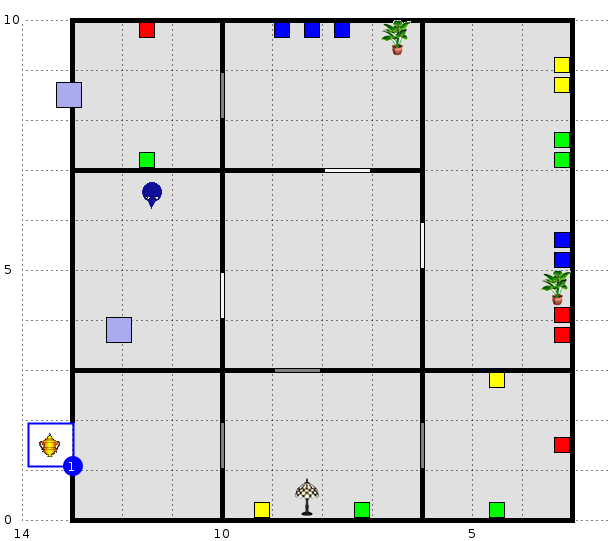
\includegraphics[width=0.7\textwidth]{Images/experiment-world-2}
	\caption{Map of the evaluation world 1.}
	\label{fig:exper-world1}
\end{figure}

\begin{figure}[!htbp]
  \centering
	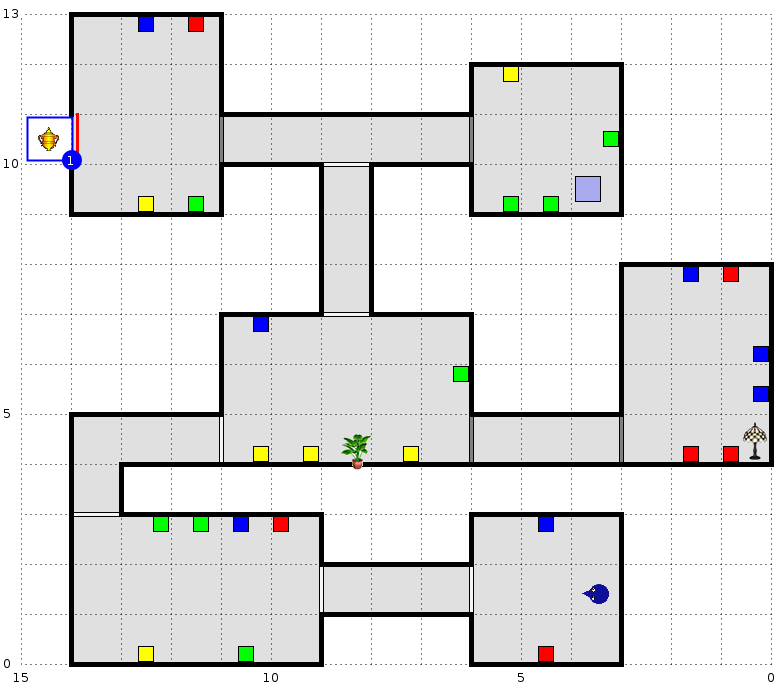
\includegraphics[width=0.7\textwidth]{Images/experiment-world-3}
	\caption{Map of the evaluation world 2.}
	\label{fig:exper-world2}
\end{figure}

\begin{figure}[!htbp]
  \centering
	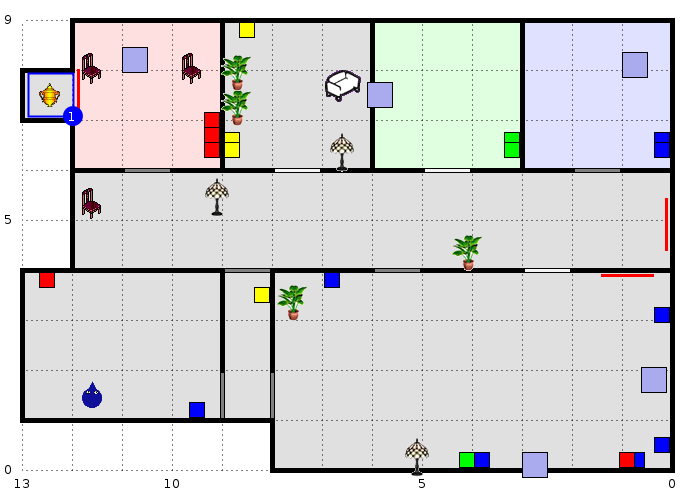
\includegraphics[width=0.7\textwidth]{Images/experiment-world-4}
	\caption{Map of the evaluation world 3.}
	\label{fig:exper-world3}
\end{figure}

\begin{figure}[!htbp]
  \centering
	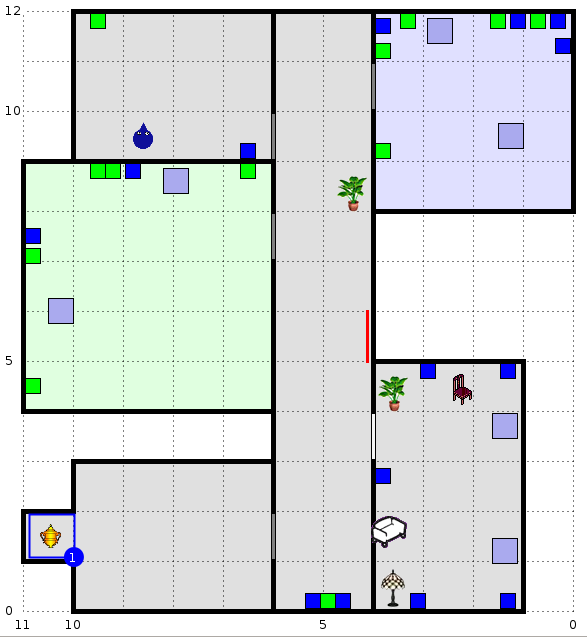
\includegraphics[width=0.7\textwidth]{Images/experiment-world-5}
	\caption{Map of the evaluation world 4.}
	\label{fig:exper-world4}
\end{figure}

I have called the two NLG systems Alpha and Beta. Since they are almost identical except for a REG strategy for the buttons, I will describe the Alpha system and simply point out the differences between it and Beta system, at the end of the description. As was previously mentioned in Chapter \ref{chap:ml}, the NLG systems are inspired by the analysis of S-GIVE dataset. Even though S-GIVE dataset is of a spoken word, I managed to transform some ideas from the spoken data to the written instructions.

Because the final systems are not subjects of this thesis, but merely a device to examine a NLP phenomenon, I will stick to high-level descriptions of the ideas behind them and avoid exhaustive software engineering description, such as class diagrams and similar devices.

First thing I would like to address is the timing. In spoken S-GIVE scenario the IG knows when the IF heard the RE. That's is however unknown for written instructions. I've partially solved this problem by estimating the timing with an average reading speed of 150 words per minute. This can of course affect the task proficiency because of the personal differences in reading speed and the effect of learning, but it is not easily solved in the framework I was using.

For the direction giving, Alpha system uses 4 directions. The were heavily used in S-GIVE dataset even though sometimes enhanced by adjectives. The directions are simple: in front of the IF, left, right and behind the IF; all from the IF point of view. In conjunction with RE which use relations between world's entities, these 4 directions are sufficient to describe the path for IF. Suppose we consider $0^{\circ}$ a direction the IF is facing, then I've chosen the limits for the 4 directions as follows: in front $\langle-35^{\circ},35^{\circ}\rangle$, right $(35^{\circ},145^{\circ})$, behind $\langle145^{\circ},-145^{\circ}\rangle$ and left $(-145^{\circ},-35^{\circ})$. The system uses them as in the following example: ``Press the green button on your left.''

Before focusing on RE to the target button, I will report on how I implemented navigating through the rooms. In a relatively simple scenarios with rooms and mainly straight corridors, the system can simply create a RE for the door leading to the next planned room, once the IF entered a new room. Adding verbs of movement such as ``go'' to this RE is a simple, yet in the S-GIVE dataset common method for navigating in GIVE scenario. Example of such sentence is: ``Go through the door in front of you.'' The only complication is that with only 4 directions, other doors can be present in the same direction as the target door. I've solved this by another RE, identifying the target door using its relative position in the group of distracting doors: ``The door closest to you.'' Whenever this specification is needed, I've also added positive feedback when the IF is heading towards the correct doors and negative feedback if he/she enters a wrong room. I have also enhanced this subsystem by two additional improvements commonly seen in S-GIVE dataset.

First, when IF is only passing through the room on his way to a next one, I modified the language realization to take advantage of that fact. The system will produce expressions such as: ``Make a left.'' or ``Keep going straight.'' This adds variability to the NLG system and makes it more human-like.

Second, I exploited the room memory, first presented in Section \ref{sec:room-memory-ml}. When IF is immediately returning to the room he/she was just in and the time elapsed since he/she was there is not large (less than 20 seconds), the system will produce an expression such as: ``Go back to the room you were just in.'' This addition not only increase human-likeness, but I would argue also has an impact on the task efficiency, since it avoids a lot of problems in standard method described above.

The most complicated task are REs to a target button. This is where the systems Alpha and Beta differ. Once IF enters the room where a button needs to be pressed, the systems decide whether a reference containing the color of the button and the direction to the button will uniquely identifies the target button. That is, whether there are distracting buttons of the same color in the same direction. If there are none, both systems simply generate a RE like this one: ``Press the green button behind you.'' However, if this (first) RE would not uniquely identify the button, additional information must be provided. The additional information picks out the target button from the group of distractors. That is done either through a landmark, which I have placed in worlds so it is possible in most cases or it is done in a similar way the door specifying RE were created. Both systems are flexible enough to be able to provide unique identification to a substantial number of cases.

The system Beta will present that additional information as part of the first RE. System Alpha, on the other hand, separates this additional information to a new RE, which is not presented immediately. The Alpha system waits until the target button is visible and only then presents the second RE. Since the first RE contains direction, it is presumed the IF will start moving towards the target button.

In cases where additional information is needed, both systems provide positive feedback when the IF is close and looking at the target button, measured by multiplying the distance between the IF and target button and the angle between them and compared to a threshold. Once a button was pressed, either positive or negative feedback is generated, depending whether IF pressed the correct button.

That concludes the high-level overview of the Alpha and Beta systems. I'll know present the results of the experiment.

\section{Results}
I've recruited $X$ colleagues and friends, mostly university students. They all had atleast basic knowledge of English language to understand the instructions. The participants together played $Z$ valid games on 4 evaluation worlds.

Overall $Y$ cases, where a target button has to be specified, were recorded. Of those $A$ were handled by Alpha system and $B$ were handled by Beta system. The means and standard deviations for the two systems can be found in table \ref{tab:meanexper}.

\begin{table}[!htbp]
 \centering
\begin{tabular}{lcc}
\toprule
System   & Average (s) & SD (s)  \\
\midrule
Alpha   & $m1$ & $std1$ \\
Beta 	& $m2$ & $std2$ \\
\bottomrule
\end{tabular}
\caption{Results of the experiment.}
\label{tab:meanexper}
\end{table}

The t-test statistics for independent two-tailed t-test is $Z$ with p-value of $p$. Therefore there isn't sufficient evidence to refuse the null hypothesis that the mean times between a first reference and the button press are equal for Alpha and Beta systems.

This experiment was only testing very specific reference splitting. The first reference always contained the position and color of the button. In case of system Beta it also contained relative position in a group of distractors or to a landmark. For system Alpha that last specification reference was delayed until the target button was visible. Because of the written instruction, the splitting system Alpha had a small disadvantage, since the second reference in some cases had to wait for the first one to finish, which slowed the referencing down. It would be interesting to explore the splitting in other scenarios and possibly in spoken navigation. But that was beyond scope of this thesis.

Based on the result, I would argue that the strategy of splitting reference is a language device to reduce complexity of REs in complex environments, which however does not significantly affects the task performance. It is an interesting phenomenon which I believe would be worth exploring for REG research.